% =========================================================
% Algebraic Structures — Functions as Transformations
% =========================================================
% Functions are treated here as transformations and structure maps.
% The focus is algebraic: injectivity = left-cancellability,
% surjectivity = solvability, bijection = reversible transformation.
% Set-theoretic foundations assumed from Volume I.

\section{Functions as Transformations}

% ---------------------------------------------------------
% TOOLKIT
% ---------------------------------------------------------
\begin{tcolorbox}[colback=gray!6, colframe=gray!40, arc=2pt,
  left=6pt, right=6pt, top=4pt, bottom=4pt,
  title={\small\textbf{Functions — Algebraic Quick Reference}},
  fonttitle=\small\bfseries]
\small
\begin{tabular}{l l l}
\toprule
\textbf{Concept} & \textbf{Algebraic meaning} & \textbf{Detail} \\
\midrule
Function          & Left-total, right-unique relation                     & \hyperref[def:alg-function]{↓} \\
Domain / Codomain & $\dom(f) = A$,\; $\cod(f) = B$ for $f : A \to B$     & \hyperref[def:alg-function]{↓} \\
Image             & $\im(f) = \{f(a) \mid a \in A\} \subseteq B$         & \hyperref[def:alg-image]{↓} \\
Image of a set    & $f(S) = \{f(a) \mid a \in S\}$ for $S \subseteq A$   & \hyperref[def:alg-image]{↓} \\
Preimage          & $f^{-1}(T) = \{a \in A \mid f(a) \in T\}$            & \hyperref[def:alg-image]{↓} \\
Fiber             & $f^{-1}(\{b\})$: preimage of a single element         & \hyperref[def:alg-fiber]{↓} \\
Graph             & $\{(a, f(a)) \mid a \in A\} \subseteq A \times B$    & \hyperref[def:alg-graph]{↓} \\
Injective         & Left-cancellable: $f \circ g = f \circ h \Rightarrow g = h$ & \hyperref[def:alg-injective]{↓} \\
Surjective        & $f(x) = b$ is always solvable                        & \hyperref[def:alg-surjective]{↓} \\
Bijective         & Invertible transformation                             & \hyperref[def:alg-bijective]{↓} \\
Isomorphism       & Bijective homomorphism; $A \cong B$                   & \hyperref[def:isomorphism]{↓} \\
Monomorphism      & Injective homomorphism; embeds $A$ into $B$           & \hyperref[def:monomorphism]{↓} \\
Epimorphism       & Surjective homomorphism; covers $B$                   & \hyperref[def:epimorphism]{↓} \\
Homomorphism      & Structure-preserving map $f : A \to B$                & \hyperref[def:homomorphism]{↓} \\
Endomorphism      & Homomorphism $f : A \to A$; $\mathrm{End}(A)$ a monoid & \hyperref[def:endomorphism]{↓} \\
Automorphism      & Bijective endomorphism; $\mathrm{Aut}(A)$ a group     & \hyperref[def:automorphism]{↓} \\
Identity          & Neutral element for composition; $\mathrm{id}_A(a)=a$ & \hyperref[def:alg-identity]{↓} \\
Inclusion map     & $\iota : A \hookrightarrow B$, $\iota(a)=a$, for $A \subseteq B$ & \hyperref[def:alg-inclusion]{↓} \\
Composition       & $(g \circ f)(a) = g(f(a))$                           & \hyperref[def:alg-composition]{↓} \\
Left inverse      & $g \circ f = \mathrm{id}_A$; exists iff $f$ injective  & \hyperref[def:alg-left-inverse]{↓} \\
Right inverse     & $f \circ h = \mathrm{id}_B$; exists iff $f$ surjective & \hyperref[def:alg-left-inverse]{↓} \\
Inverse           & Two-sided; exists iff $f$ bijective                  & \hyperref[def:alg-inverse]{↓} \\
Restriction       & $f|_C : C \to B$, domain cut to $C \subseteq A$      & \hyperref[def:alg-restriction]{↓} \\
Extension         & $g : A' \to B$ with $g|_A = f$, domain enlarged      & \hyperref[def:alg-restriction]{↓} \\
\bottomrule
\end{tabular}
\end{tcolorbox}

\vspace{1em}

% ---------------------------------------------------------
% Function as a special relation
% ---------------------------------------------------------

\begin{tcolorbox}[colback=propbox, colframe=propborder, arc=2pt,
  left=6pt, right=6pt, top=4pt, bottom=4pt,
  title={\small\textbf{Definition (Function)}},
  fonttitle=\small\bfseries]
\label{def:alg-function}
Let $A$ and $B$ be sets.
A \emph{function} from $A$ to $B$ is a binary relation $f \subseteq A \times B$
that is:
\begin{enumerate}[label=(\roman*)]
  \item \emph{left-total}: every element of $A$ appears as a first coordinate,
        \[
          \forall a \in A,\quad \exists b \in B,\quad (a,b) \in f;
        \]
  \item \emph{right-unique}: no element of $A$ is paired with two distinct
        elements of $B$,
        \[
          (a,b_1) \in f \;\land\; (a,b_2) \in f \;\Rightarrow\; b_1 = b_2.
        \]
\end{enumerate}
We write $f : A \to B$ and $f(a) = b$ in place of $(a,b) \in f$.
The set $A$ is the \emph{domain} $\dom(f)$ and $B$ is the \emph{codomain}
$\cod(f)$.
\end{tcolorbox}

\begin{remark}[Fully quantified form]
$f : A \to B$ is a function
$\;\iff\;$
$(\forall a \in A)\;(\exists!\, b \in B)\; (a,b) \in f$.
\end{remark}

\begin{remark}[Function as special relation]
Every function is a relation, but not every relation is a function.
Left-totality rules out relations that leave some input without an output.
Right-uniqueness rules out relations that assign multiple outputs to one input.
Together they force exactly one output per input — the defining property of
a function.
\end{remark}

\begin{remark}[Algebraic perspective]
Once the relational grounding is fixed, the algebraic interest shifts to what
$f$ \emph{does}: how it interacts with composition, whether it can be
inverted, and whether it preserves structure on $A$ and $B$.
\end{remark}

% ---------------------------------------------------------
% Image / Preimage / Fiber
% ---------------------------------------------------------

\begin{tcolorbox}[colback=propbox, colframe=propborder, arc=2pt,
  left=6pt, right=6pt, top=4pt, bottom=4pt,
  title={\small\textbf{Definition (Image / Preimage / Fiber)}},
  fonttitle=\small\bfseries]
\label{def:alg-image}
Let $f : A \to B$, $S \subseteq A$, and $T \subseteq B$.
\begin{enumerate}[label=(\roman*)]
  \item The \emph{image of $f$} is
        \[
          \im(f) \;:=\; \{\, b \in B \mid \exists a \in A,\; f(a) = b \,\}.
        \]
  \item The \emph{image of $S$ under $f$} is
        \[
          f(S) \;:=\; \{\, f(a) \mid a \in S \,\}.
        \]
        Note $f(A) = \im(f)$.
  \item The \emph{preimage of $T$ under $f$} is
        \[
          f^{-1}(T) \;:=\; \{\, a \in A \mid f(a) \in T \,\}.
        \]
\end{enumerate}
\end{tcolorbox}

\begin{remark}[Fully quantified form]
$\im(f) = \{b \in B \mid (\exists a \in A)\; f(a) = b\}$.
$f(S) = \{b \in B \mid (\exists a \in S)\; f(a) = b\}$.
$f^{-1}(T) = \{a \in A \mid f(a) \in T\}$.
\end{remark}

\begin{remark}[Preimage notation warning]
$f^{-1}(T)$ is defined for \emph{every} function $f$, whether or not $f$
is injective or bijective.
It does not denote an inverse function — it is the set of all inputs that
map into $T$.
\end{remark}

\begin{tcolorbox}[colback=propbox, colframe=propborder, arc=2pt,
  left=6pt, right=6pt, top=4pt, bottom=4pt,
  title={\small\textbf{Definition (Fiber)}},
  fonttitle=\small\bfseries]
\label{def:alg-fiber}
The \emph{fiber of $f$ over $b \in B$} is the preimage of the singleton:
\[
  f^{-1}(\{b\}) \;=\; \{\, a \in A \mid f(a) = b \,\}.
\]
\end{tcolorbox}

\begin{remark}[Fully quantified form]
$f^{-1}(\{b\}) = \{a \in A \mid f(a) = b\}$.
\end{remark}

\begin{remark}[Fibers and injectivity]
Injectivity: each fiber has at most one element.
Surjectivity: every fiber is nonempty.
Bijectivity: every fiber has exactly one element.
The fibers of $f$ partition $A$ into the equivalence classes of the
relation $a_1 \sim_f a_2 \iff f(a_1) = f(a_2)$.
This equivalence relation is the kernel of $f$, and will reappear
as the kernel of a homomorphism in abstract algebra.
\end{remark}

% ---------------------------------------------------------
% Graph
% ---------------------------------------------------------

\begin{tcolorbox}[colback=propbox, colframe=propborder, arc=2pt,
  left=6pt, right=6pt, top=4pt, bottom=4pt,
  title={\small\textbf{Definition (Graph of a Function)}},
  fonttitle=\small\bfseries]
\label{def:alg-graph}
The \emph{graph} of $f : A \to B$ is the subset
\[
  \Gamma_f \;:=\; \{\,(a, f(a)) \mid a \in A\,\} \;\subseteq\; A \times B.
\]
\end{tcolorbox}

\begin{remark}[Fully quantified form]
$\Gamma_f = \{(a,b) \in A \times B \mid b = f(a)\}$.
\end{remark}

\begin{remark}[Graph and the relational definition]
The graph $\Gamma_f$ is precisely the relation $f \subseteq A \times B$
of the relational definition above.
A subset $G \subseteq A \times B$ is the graph of some function
$A \to B$ if and only if it is left-total and right-unique.
Functions and their graphs are the same object — the graph notation simply
makes the set-theoretic representation explicit.
\end{remark}

% ---------------------------------------------------------
% Vocabulary diagram
% ---------------------------------------------------------

\begin{figure}[h]
\centering
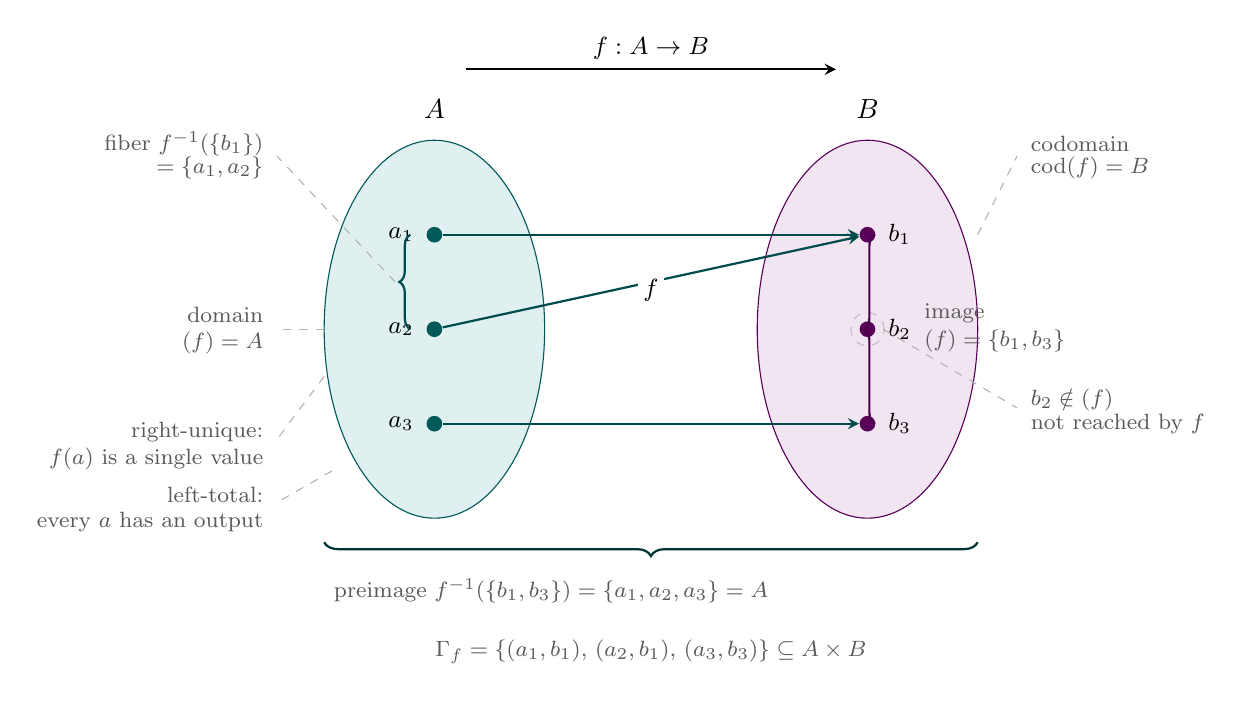
\begin{tikzpicture}[
    >=stealth,
    dot/.style     = {circle, fill, inner sep=2pt},
    teal/.style    = {draw=teal!70!black,  fill=teal!12},
    purple/.style  = {draw=violet!70!black, fill=violet!10},
    lbl/.style     = {font=\small},
    ann/.style     = {font=\footnotesize, text=gray!70!black},
    leader/.style  = {gray!60, dashed, thin},
    arr/.style     = {->, thick, teal!60!black},
    brace/.style   = {decorate,
                      decoration={brace, amplitude=4pt, raise=3pt},
                      thick, violet!60!black}
  ]

  % --- blobs ---
  \draw[teal]   (0,0)   ellipse (1.4cm and 2.4cm);
  \draw[purple] (5.5,0) ellipse (1.4cm and 2.4cm);

  % blob labels
  \node[font=\normalsize\bfseries] at (0,    2.8) {$A$};
  \node[font=\normalsize\bfseries] at (5.5,  2.8) {$B$};

  % --- elements of A ---
  \node[dot, teal!70!black] (a1) at (0,  1.2) {};
  \node[dot, teal!70!black] (a2) at (0,  0)   {};
  \node[dot, teal!70!black] (a3) at (0, -1.2) {};

  \node[lbl, left=4pt] at (a1) {$a_1$};
  \node[lbl, left=4pt] at (a2) {$a_2$};
  \node[lbl, left=4pt] at (a3) {$a_3$};

  % --- elements of B ---
  \node[dot, violet!70!black] (b1) at (5.5,  1.2) {};
  \node[dot, violet!70!black] (b2) at (5.5,  0)   {};
  \node[dot, violet!70!black] (b3) at (5.5, -1.2) {};

  \node[lbl, right=4pt] at (b1) {$b_1$};
  \node[lbl, right=4pt] at (b2) {$b_2$};
  \node[lbl, right=4pt] at (b3) {$b_3$};

  % b2 not in image: dashed ring
  \draw[gray!50, dashed, thin] (b2) circle (6pt);

  % --- arrows ---
  \draw[arr] (a1) -- (b1);
  \draw[arr] (a2) -- (b1);   % two inputs to b1 => not injective
  \draw[arr] (a3) -- (b3);

  % f label on central arrow
  \node[fill=white, inner sep=2pt, font=\small\bfseries] at (2.75, 0.5) {$f$};

  % --- top-level f : A -> B arrow ---
  \draw[->, thick] (0.4, 3.3) -- node[above, font=\small\bfseries] {$f : A \to B$} (5.1, 3.3);

  % ===  LEFT SIDE ANNOTATIONS ===

  % domain
  \draw[leader] (-1.4, 0) -- (-2.0, 0);
  \node[ann, anchor=east] at (-2.05, 0.18) {domain};
  \node[ann, anchor=east] at (-2.05,-0.18) {$\dom(f) = A$};

  % left-total
  \draw[leader] (-1.3,-1.8) -- (-2.0,-2.2);
  \node[ann, anchor=east] at (-2.05,-2.1) {left-total:};
  \node[ann, anchor=east] at (-2.05,-2.45) {every $a$ has an output};

  % right-unique -- left margin, below domain, clear of everything
  \draw[leader] (-1.4, -0.6) -- (-2.0, -1.4);
  \node[ann, anchor=east] at (-2.05,-1.3)  {right-unique:};
  \node[ann, anchor=east] at (-2.05,-1.65) {$f(a)$ is a single value};

  % === RIGHT SIDE ANNOTATIONS ===

  % codomain  -- top right, well clear of image
  \draw[leader] (6.9,  1.2) -- (7.4,  2.2);
  \node[ann, anchor=west] at (7.45, 2.35) {codomain};
  \node[ann, anchor=west] at (7.45, 2.05) {$\mathrm{cod}(f) = B$};

  % image -- mid right, below codomain
  \draw[brace] (5.7, -1.2) -- (5.7,  1.2);
  \node[ann, anchor=west] at (6.1,  0.2) {image};
  \node[ann, anchor=west] at (6.1, -0.15) {$\im(f) = \{b_1, b_3\}$};

  % b2 not in image
  \draw[leader] (5.7, 0) -- (7.4, -1.0);
  \node[ann, anchor=west] at (7.45,-0.9)  {$b_2 \notin \im(f)$};
  \node[ann, anchor=west] at (7.45,-1.2)  {not reached by $f$};

  % fiber of b1: curly brace on LEFT blob, spanning a1 and a2
  \draw[decorate,
        decoration={brace, amplitude=4pt, raise=3pt},
        thick, teal!60!black]
    (-0.2, 0) -- (-0.2, 1.2);
  \draw[leader] (-0.5, 0.6) -- (-2.0, 2.2);
  \node[ann, anchor=east] at (-2.05, 2.35) {fiber $f^{-1}(\{b_1\})$};
  \node[ann, anchor=east] at (-2.05, 2.05) {$= \{a_1, a_2\}$};

  % preimage of T = {b1, b3}  -- bracket under both blobs
  \draw[decorate,
        decoration={brace, amplitude=5pt, raise=3pt, mirror},
        thick, teal!40!black]
    (-1.4,-2.6) -- (6.9,-2.6);
  % label anchored left so it clears the right-unique text
  \node[ann, anchor=north west] at (-1.4,-3.05)
    {preimage $f^{-1}(\{b_1,b_3\}) = \{a_1,a_2,a_3\} = A$};

  % graph label
  \node[ann] at (2.75,-4.1)
    {$\Gamma_f = \{(a_1,b_1),\,(a_2,b_1),\,(a_3,b_3)\} \subseteq A \times B$};

\end{tikzpicture}
\caption{Vocabulary of a function $f : A \to B$.
  Arrows show $f(a_1)=f(a_2)=b_1$ and $f(a_3)=b_3$.
  The element $b_2$ is not in the image; its fiber is empty.
  The fiber over $b_1$ has two elements, showing $f$ is not injective.}
\label{fig:function-vocabulary}
\end{figure}

% ---------------------------------------------------------
% Injective / Surjective / Bijective
% ---------------------------------------------------------

\begin{tcolorbox}[colback=propbox, colframe=propborder, arc=2pt,
  left=6pt, right=6pt, top=4pt, bottom=4pt,
  title={\small\textbf{Definition (Injective)}},
  fonttitle=\small\bfseries]
\label{def:alg-injective}
$f : A \to B$ is \emph{injective} (one-to-one) if distinct inputs
produce distinct outputs:
\[
  \forall a_1, a_2 \in A,\quad
  f(a_1) = f(a_2) \;\Rightarrow\; a_1 = a_2.
\]
Equivalently, $f$ is \emph{left-cancellable}: for all functions
$g, h : C \to A$,
\[
  f \circ g = f \circ h \;\Rightarrow\; g = h.
\]
\end{tcolorbox}

\begin{remark}[Fully quantified form]
$(\forall a_1, a_2 \in A)\;[f(a_1) = f(a_2) \Rightarrow a_1 = a_2]$.
\end{remark}

\begin{remark}[Algebraic meaning]
Injectivity says $f$ never collapses distinct elements.
In algebraic contexts, an injective structure-preserving map (homomorphism)
embeds one structure inside another without identification.
The left-cancellability formulation makes this precise:
$f$ does not lose information, so pre-composing with $f$ can always be
undone.
\end{remark}

\begin{tcolorbox}[colback=propbox, colframe=propborder, arc=2pt,
  left=6pt, right=6pt, top=4pt, bottom=4pt,
  title={\small\textbf{Definition (Surjective)}},
  fonttitle=\small\bfseries]
\label{def:alg-surjective}
$f : A \to B$ is \emph{surjective} (onto) if every element of $B$
is achieved as an output:
\[
  \forall b \in B,\quad \exists a \in A,\quad f(a) = b.
\]
Equivalently, $f$ is \emph{right-cancellable}: for all functions
$g, h : B \to C$,
\[
  g \circ f = h \circ f \;\Rightarrow\; g = h.
\]
\end{tcolorbox}

\begin{remark}[Fully quantified form]
$(\forall b \in B)\;(\exists a \in A)\; f(a) = b$.
\end{remark}

\begin{remark}[Algebraic meaning]
Surjectivity says the equation $f(a) = b$ has a solution for every $b$.
This is the algebraic notion of \emph{solvability}.
In group theory, a surjective homomorphism allows every element of the
target group to be ``reached'' — it is the condition for a
quotient construction to be valid.
\end{remark}

\begin{tcolorbox}[colback=propbox, colframe=propborder, arc=2pt,
  left=6pt, right=6pt, top=4pt, bottom=4pt,
  title={\small\textbf{Definition (Bijective)}},
  fonttitle=\small\bfseries]
\label{def:alg-bijective}
$f : A \to B$ is \emph{bijective} if it is both injective and surjective.
A bijection is a \emph{one-to-one correspondence} between $A$ and $B$.
\end{tcolorbox}

\begin{remark}[Fully quantified form]
$f$ is bijective
$\;\iff\;$
$(\forall a_1,a_2 \in A)\,[f(a_1)=f(a_2)\Rightarrow a_1=a_2]$
$\;\land\;$
$(\forall b \in B)\,(\exists a \in A)\,[f(a)=b]$.
\end{remark}

\begin{remark}[Algebraic meaning]
A bijection is a \emph{reversible transformation}: it identifies $A$ and $B$
as sets up to renaming.
A bijection that also preserves algebraic structure is an isomorphism —
defined precisely in the morphisms section below.
\end{remark}

% ---------------------------------------------------------
% Morphisms
% ---------------------------------------------------------

\subsection{Morphisms}

% ---------------------------------------------------------
% TOOLKIT — Morphisms
% ---------------------------------------------------------
\begin{tcolorbox}[colback=gray!6, colframe=gray!40, arc=2pt,
  left=6pt, right=6pt, top=4pt, bottom=4pt,
  title={\small\textbf{Morphisms — Quick Reference}},
  fonttitle=\small\bfseries]
\small
\begin{tabular}{l l l l}
\toprule
\textbf{Name} & \textbf{Domain / Codomain} & \textbf{Conditions} & \textbf{Detail} \\
\midrule
Homomorphism  & $f : A \to B$   & Structure-preserving                  & \hyperref[def:homomorphism]{↓} \\
Monomorphism  & $f : A \to B$   & Homomorphism + injective              & \hyperref[def:monomorphism]{↓} \\
Epimorphism   & $f : A \to B$   & Homomorphism + surjective             & \hyperref[def:epimorphism]{↓} \\
Isomorphism   & $f : A \to B$   & Homomorphism + bijective; $A \cong B$ & \hyperref[def:isomorphism]{↓} \\
Endomorphism  & $f : A \to A$   & Homomorphism; domain = codomain       & \hyperref[def:endomorphism]{↓} \\
Automorphism  & $f : A \to A$   & Isomorphism; domain = codomain        & \hyperref[def:automorphism]{↓} \\
\bottomrule
\end{tabular}
\end{tcolorbox}

\vspace{0.5em}

\begin{center}
\small
\begin{tabular}{r | c c}
                    & $A \to B$        & $A \to A$       \\
\hline
Structure-preserving & homomorphism     & endomorphism    \\
+ bijective          & isomorphism      & automorphism    \\
\end{tabular}
\end{center}

\vspace{1em}

% ---------------------------------------------------------
% Homomorphism
% ---------------------------------------------------------

\begin{tcolorbox}[colback=propbox, colframe=propborder, arc=2pt,
  left=6pt, right=6pt, top=4pt, bottom=4pt,
  title={\small\textbf{Definition (Homomorphism)}},
  fonttitle=\small\bfseries]
\label{def:homomorphism}
Let $A$ and $B$ be sets each carrying algebraic structure
(operations, relations, or both).
A function $f : A \to B$ is a \emph{homomorphism} if it
\emph{preserves structure}: every operation and relation on $A$
corresponds to its counterpart on $B$ under $f$.

For a single binary operation $\star$, this means:
\[
  \forall a_1, a_2 \in A,\quad f(a_1 \star a_2) = f(a_1) \star f(a_2).
\]
For an order relation $\leq$, this means:
\[
  \forall a_1, a_2 \in A,\quad a_1 \leq a_2 \;\Rightarrow\; f(a_1) \leq f(a_2).
\]
The precise condition depends on the structure carried by $A$ and $B$;
the general pattern is always: $f$ commutes with every operation and
respects every relation.
\end{tcolorbox}

\begin{remark}[Fully quantified form]
For a binary operation $\star$:
$(\forall a_1, a_2 \in A)\; f(a_1 \star a_2) = f(a_1) \star f(a_2)$.
\end{remark}

\begin{remark}[Algebraic meaning]
A homomorphism is a \emph{structure-preserving map}: it carries the
algebraic relationships in $A$ faithfully into $B$, but it may collapse
distinct elements (if not injective) or fail to reach all of $B$
(if not surjective).
The image $f(A)$ is always a substructure of $B$ — a copy of (a quotient
of) $A$ sitting inside $B$.
The \emph{kernel} of a homomorphism — the set of elements mapping to the
identity — measures how much the map collapses; its structure governs the
First Isomorphism Theorem.
Both the kernel and the isomorphism theorems are developed in abstract
algebra; what is recorded here is the foundational definition.
\end{remark}

\begin{remark}[Every isomorphism is a homomorphism; not conversely]
A homomorphism need not be injective or surjective.
The map $f : \mathbb{Z} \to \mathbb{Z}/n\mathbb{Z}$, $f(k) = k \bmod n$,
is a surjective homomorphism that is not injective.
The map $f : \mathbb{Z} \to \mathbb{Z}$, $f(k) = 2k$, is an injective
homomorphism that is not surjective.
The full classification of homomorphisms by their bijectivity properties
is the content of the next three definitions.
\end{remark}

% ---------------------------------------------------------
% Monomorphism / Epimorphism
% ---------------------------------------------------------

\begin{tcolorbox}[colback=propbox, colframe=propborder, arc=2pt,
  left=6pt, right=6pt, top=4pt, bottom=4pt,
  title={\small\textbf{Definition (Monomorphism / Epimorphism)}},
  fonttitle=\small\bfseries]
\label{def:monomorphism}
\label{def:epimorphism}
Let $f : A \to B$ be a homomorphism.
\begin{enumerate}[label=(\roman*)]
  \item $f$ is a \emph{monomorphism} if $f$ is injective:
        \[
          f(a_1) = f(a_2) \;\Rightarrow\; a_1 = a_2.
        \]
        A monomorphism \emph{embeds} $A$ into $B$ without identification.
  \item $f$ is an \emph{epimorphism} if $f$ is surjective:
        \[
          \forall b \in B,\quad \exists a \in A,\quad f(a) = b.
        \]
        An epimorphism \emph{covers} $B$ — every element of $B$ is reached.
\end{enumerate}
\end{tcolorbox}

\begin{remark}[Fully quantified form]
Monomorphism: $(\forall a_1, a_2 \in A)\;[f(a_1) = f(a_2) \Rightarrow a_1 = a_2]$,
with $f$ a homomorphism.
Epimorphism: $(\forall b \in B)\;(\exists a \in A)\;[f(a) = b]$,
with $f$ a homomorphism.
\end{remark}

\begin{remark}[Mono- and epi- vs.\ injective and surjective]
In the category of sets, monomorphism coincides with injective and
epimorphism coincides with surjective.
In other categories (rings, topological spaces) this can fail:
there exist epimorphisms of rings that are not surjective functions.
At this pre-structure level the set-theoretic and categorical meanings agree;
the distinction matters only when working inside a specific category.
\end{remark}

% ---------------------------------------------------------
% Isomorphism
% ---------------------------------------------------------

\begin{tcolorbox}[colback=propbox, colframe=propborder, arc=2pt,
  left=6pt, right=6pt, top=4pt, bottom=4pt,
  title={\small\textbf{Definition (Isomorphism)}},
  fonttitle=\small\bfseries]
\label{def:isomorphism}
\label{def:alg-isomorphism}
A homomorphism $f : A \to B$ is an \emph{isomorphism} if it is bijective
— equivalently, if it is both a monomorphism and an epimorphism.
When an isomorphism $f : A \to B$ exists we say $A$ and $B$ are
\emph{isomorphic} and write $A \cong B$.
\end{tcolorbox}

\begin{remark}[Fully quantified form]
$f : A \to B$ is an isomorphism
$\;\iff\;$
$f$ is a homomorphism
$\;\land\;$
$(\forall a_1,a_2 \in A)\,[f(a_1)=f(a_2) \Rightarrow a_1=a_2]$
$\;\land\;$
$(\forall b \in B)\,(\exists a \in A)\,[f(a)=b]$.
\end{remark}

\begin{remark}[Algebraic meaning]
Isomorphic structures are algebraically identical — they differ only in
the names of their elements.
The inverse $f^{-1}$ of an isomorphism is itself an isomorphism.
\end{remark}

\begin{remark}[Isomorphism is an equivalence relation]
The relation $\cong$ on a collection of structures is an equivalence relation:
reflexive ($A \cong A$ via $\mathrm{id}_A$),
symmetric ($A \cong B \Rightarrow B \cong A$ via $f^{-1}$),
and transitive ($A \cong B$ and $B \cong C \Rightarrow A \cong C$ via
$g \circ f$).
\end{remark}

% ---------------------------------------------------------
% Endomorphism
% ---------------------------------------------------------

\begin{tcolorbox}[colback=propbox, colframe=propborder, arc=2pt,
  left=6pt, right=6pt, top=4pt, bottom=4pt,
  title={\small\textbf{Definition (Endomorphism)}},
  fonttitle=\small\bfseries]
\label{def:endomorphism}
An \emph{endomorphism} of $A$ is a homomorphism from $A$ to itself:
\[
  f : A \to A \quad \text{structure-preserving, not necessarily bijective.}
\]
The set of all endomorphisms of $A$ is denoted $\mathrm{End}(A)$.
\end{tcolorbox}

\begin{remark}[Fully quantified form]
$f \in \mathrm{End}(A)$
$\;\iff\;$
$f : A \to A$ is a homomorphism.
\end{remark}

\begin{remark}[Algebraic meaning]
$\mathrm{End}(A)$ is closed under composition: the composite of two
structure-preserving self-maps is again structure-preserving.
Together with $\mathrm{id}_A$ as neutral element, this makes
$(\mathrm{End}(A), \circ)$ a \emph{monoid}.
Automorphisms are precisely the invertible endomorphisms:
$\mathrm{Aut}(A) = \{f \in \mathrm{End}(A) \mid f \text{ is bijective}\}$.
\end{remark}

% ---------------------------------------------------------
% Automorphism
% ---------------------------------------------------------

\begin{tcolorbox}[colback=propbox, colframe=propborder, arc=2pt,
  left=6pt, right=6pt, top=4pt, bottom=4pt,
  title={\small\textbf{Definition (Automorphism)}},
  fonttitle=\small\bfseries]
\label{def:automorphism}
\label{def:alg-automorphism}
An \emph{automorphism} of $A$ is a bijective endomorphism of $A$ —
equivalently, an isomorphism from $A$ to itself:
\[
  f : A \xrightarrow{\;\sim\;} A.
\]
The set of all automorphisms of $A$ is denoted $\mathrm{Aut}(A)$.
\end{tcolorbox}

\begin{remark}[Fully quantified form]
$f \in \mathrm{Aut}(A)$
$\;\iff\;$
$f \in \mathrm{End}(A)$ and $f$ is bijective
$\;\iff\;$
$f : A \to A$ is an isomorphism.
\end{remark}

\begin{remark}[Algebraic meaning]
An automorphism is a \emph{symmetry} of $A$: a relabelling of its elements
that leaves every algebraic relationship intact.
$\mathrm{Aut}(A)$ is closed under composition and inverses, and contains
$\mathrm{id}_A$ — making $(\mathrm{Aut}(A), \circ)$ a \emph{group},
the automorphism group of $A$.
This group encodes all the internal symmetry of the structure, and is one
of the first and most important groups encountered in abstract algebra.
\end{remark}

% ---------------------------------------------------------
% Composition
% ---------------------------------------------------------

\begin{tcolorbox}[colback=propbox, colframe=propborder, arc=2pt,
  left=6pt, right=6pt, top=4pt, bottom=4pt,
  title={\small\textbf{Definition (Composition)}},
  fonttitle=\small\bfseries]
\label{def:alg-composition}
Let $f : A \to B$ and $g : B \to C$.
The \emph{composition} $g \circ f : A \to C$ is the function defined by
\[
  (g \circ f)(a) \;:=\; g(f(a)) \quad \text{for all } a \in A.
\]
\end{tcolorbox}

\begin{remark}[Fully quantified form]
$(\forall a \in A)\;(g \circ f)(a) = g(f(a))$.
\end{remark}

\begin{remark}[Composition is a binary operation]
When $A = B = C$, composition is a binary operation on the set
$\mathrm{End}(A) = \{f : A \to A\}$ of all self-maps of $A$:
\[
  \circ \;:\; \mathrm{End}(A) \times \mathrm{End}(A) \to \mathrm{End}(A).
\]
This operation is \emph{associative} — $(h \circ g) \circ f = h \circ (g \circ f)$
— but not in general commutative.
The structure $(\mathrm{End}(A), \circ)$ is the first example of a monoid
that will appear when abstract algebra begins.
\end{remark}

% ---------------------------------------------------------
% Identity
% ---------------------------------------------------------

\begin{tcolorbox}[colback=propbox, colframe=propborder, arc=2pt,
  left=6pt, right=6pt, top=4pt, bottom=4pt,
  title={\small\textbf{Definition (Identity Function)}},
  fonttitle=\small\bfseries]
\label{def:alg-identity}
The \emph{identity function} on $A$ is the function
$\mathrm{id}_A : A \to A$ defined by
\[
  \mathrm{id}_A(a) := a \quad \text{for all } a \in A.
\]
\end{tcolorbox}

\begin{remark}[Fully quantified form]
$(\forall a \in A)\;\mathrm{id}_A(a) = a$.
\end{remark}

\begin{remark}[Neutral element for composition]
The identity function is the \emph{neutral element} (two-sided identity)
for composition on $\mathrm{End}(A)$:
\[
  f \circ \mathrm{id}_A = f
  \qquad \text{and} \qquad
  \mathrm{id}_B \circ f = f
\]
for all $f : A \to B$.
This is the algebraic reason the identity deserves its name.
\end{remark}

% ---------------------------------------------------------
% Inclusion map
% ---------------------------------------------------------

\begin{tcolorbox}[colback=propbox, colframe=propborder, arc=2pt,
  left=6pt, right=6pt, top=4pt, bottom=4pt,
  title={\small\textbf{Definition (Inclusion Map)}},
  fonttitle=\small\bfseries]
\label{def:alg-inclusion}
Let $A \subseteq B$.
The \emph{inclusion map} $\iota : A \hookrightarrow B$ is the function
defined by
\[
  \iota(a) := a \quad \text{for all } a \in A.
\]
\end{tcolorbox}

\begin{remark}[Fully quantified form]
$(\forall a \in A)\;\iota(a) = a$, with $\iota : A \to B$ and $A \subseteq B$.
\end{remark}

\begin{remark}[Inclusion vs.\ identity]
Both send each element to itself, but they differ in codomain.
The identity $\mathrm{id}_A : A \to A$ has codomain $A$;
the inclusion $\iota : A \hookrightarrow B$ has the strictly larger codomain $B$
when $A \subsetneq B$.
The inclusion map is always injective.
When $A = B$, the inclusion and the identity coincide.
\end{remark}

% ---------------------------------------------------------
% Restriction and Extension
% ---------------------------------------------------------

\begin{tcolorbox}[colback=propbox, colframe=propborder, arc=2pt,
  left=6pt, right=6pt, top=4pt, bottom=4pt,
  title={\small\textbf{Definition (Restriction / Extension)}},
  fonttitle=\small\bfseries]
\label{def:alg-restriction}
Let $f : A \to B$ and $C \subseteq A$.
\begin{enumerate}[label=(\roman*)]
  \item The \emph{restriction of $f$ to $C$} is the function
        $f|_C : C \to B$ defined by
        \[
          f|_C(c) := f(c) \quad \text{for all } c \in C.
        \]
  \item A function $g : A' \to B$ is an \emph{extension of $f$} to $A'$
        if $A \subseteq A'$ and
        \[
          g|_A = f,
        \]
        that is, $g(a) = f(a)$ for all $a \in A$.
\end{enumerate}
\end{tcolorbox}

\begin{remark}[Fully quantified form]
Restriction: $(\forall c \in C)\; f|_C(c) = f(c)$, with $C \subseteq A$.
Extension: $(\forall a \in A)\; g(a) = f(a)$, with $A \subseteq A'$.
\end{remark}

\begin{remark}[Restriction and inclusion]
The restriction $f|_C$ is the composition $f \circ \iota$ where
$\iota : C \hookrightarrow A$ is the inclusion map.
This makes the connection between restriction and the inclusion map
precise: restricting a function is composing on the right with an inclusion.
\end{remark}

% ---------------------------------------------------------
% Inverses
% ---------------------------------------------------------

\begin{tcolorbox}[colback=propbox, colframe=propborder, arc=2pt,
  left=6pt, right=6pt, top=4pt, bottom=4pt,
  title={\small\textbf{Definition (Left Inverse / Right Inverse / Inverse)}},
  fonttitle=\small\bfseries]
\label{def:alg-left-inverse}
\label{def:alg-inverse}
Let $f : A \to B$.
\begin{enumerate}[label=(\roman*)]
  \item A function $g : B \to A$ is a \emph{left inverse} of $f$ if
        \[
          g \circ f = \mathrm{id}_A.
        \]
  \item A function $h : B \to A$ is a \emph{right inverse} of $f$ if
        \[
          f \circ h = \mathrm{id}_B.
        \]
  \item $f$ has an \emph{inverse} (is \emph{invertible}) if there exists
        $f^{-1} : B \to A$ satisfying both:
        \[
          f^{-1} \circ f = \mathrm{id}_A
          \qquad \text{and} \qquad
          f \circ f^{-1} = \mathrm{id}_B.
        \]
\end{enumerate}
\end{tcolorbox}

\begin{remark}[Fully quantified form]
Left inverse: $(\forall a \in A)\; g(f(a)) = a$.
\quad
Right inverse: $(\forall b \in B)\; f(h(b)) = b$.
\quad
Inverse: both hold simultaneously with $g = h = f^{-1}$.
\end{remark}

\begin{remark}[Inverses and bijectivity]
$f$ has a left inverse if and only if $f$ is injective.
$f$ has a right inverse if and only if $f$ is surjective.
$f$ is invertible if and only if $f$ is bijective.
The two-sided inverse, when it exists, is unique.
This is the precise algebraic meaning of reversibility:
$f^{-1}$ undoes $f$ from both sides.
\end{remark}

\begin{remark}[Asymmetry of one-sided inverses]
A left inverse of $f$ need not be unique and need not be a right inverse.
A right inverse of $f$ need not be unique and need not be a left inverse.
Only when both exist and agree do they produce the unique two-sided inverse
$f^{-1}$.
\end{remark}